\subsection{Dean}
%

% - Purpose & Problem description:
%     These first two parts give reader short details about the test case,
%     the physical phenomena involved and specify how the numerical solution will be validated
%
\subsubsection{Purpose}
%
This test case aims to verify the developpement made to take into account the wave energy dissipation induced by vegetation. When the ratio between vegetation height and water depth is important, dissipation may become non negligible.
%
\subsubsection{Description of the problem}
%
In order to carry out an analysis of the influence of plant height, vegetation field width and breaking on waves propagation, Mendez and Losada (2004) analysed the evolution of the wave height over a Dean’s shape profile \cite{dean91} defined as follows:
$$	
h=0.25(300-x)^\frac{2}{3}
$$
Where h [m] is the water depth, 0.25 the sediment scale parameter, and x=0 is the offshore boundary.

\subsubsection{Reference}
%
In this test case the prediction of the effects of vegetation is validated with the original equation and results from Mendez and Losada (2004) \cite{mendez}.
The reference file {\it fom\_dean.slf} contains the results that have been compared to \cite{mendez} in \cite{vito}.

\subsubsection{Physical parameters}
%
Two vegetation heights, dv = 1~m and 3~m and a single 100~m long vegetation field, from 50 to 150~m, are used. The number of plants per square meter is $N = 20~units/m^2$ and the plant area per unit height of vegetation is $b_v = 0.25~m.$ The bulk drag coefficient is 0.2. All these parameters are set in the Fortran user subroutine {\it QVEG}

\subsubsection{Geometry and Mesh}
%
The computational domain was composed of a flat (slope = 0.0) 2D grid with an aspect ratio of 1 (cross-shore direction):10 (along shore direction). The calculation grid size was set as 2.0 m in the wave propagation direction.
Bathymetry and mesh are shown on figure \ref{bathydean}. There are 906 nodes and 1500 triangles.
\begin{figure} [!h]
\centering
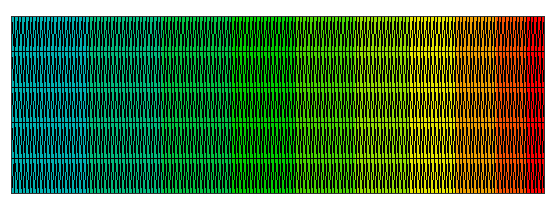
\includegraphics[scale = 0.8]{bathy.png}
%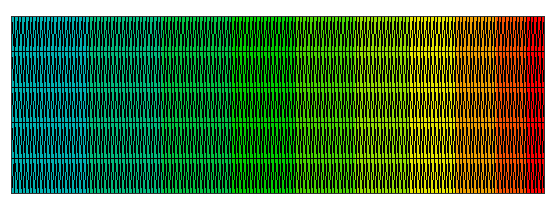
\includegraphics{bathy.png}
 \caption{depth evolution}
\label{bathydean}
\end{figure}

\subsubsection{Initial and Boundary Conditions}
%
According to the authors, the incident wave conditions imposed to TOMA\-WAC on the offshore boundary are given by $H_{rms,o} = 2.5~m$ (equivalent to significant wave height $H_s = 3.54~m$) and $T_p = 10~s$.
The incident waves are uni-directional random waves as defined in the previous section and the breaking model used is that of Thornton and Guza (1983) with  $\gamma=0.6$ (where the parameter $\gamma$  is the proportional control factor indicating the maximum water depth “Hm” compatible with water depth “d”: ).

The significant initial wave heigth was taken equal to 3.54~m with a peak frequency of 2.2~Hz. The angular distribution function follows a $\cos^{2s} \theta$ distribution with an angular spreading of 2, and a mean direction of 90.

\subsubsection{Numerical parameters}
%
The time step is of 0.1~s and the duration of the computation of 480~s. The spectro-angular mesh has 36 directions and 6 frequencies. The frequential ratio is of 1.01 and the minimum frequency of 0.0951~Hz. The frequencies are filtered to keep only the fourth one (0.1 Hz) at 90 degrees to respect the $T_p= 10~s$ imposed to the boundaries.

The spectrum tail factor was taken at 4.

\subsubsection{Results}
%
 The results from Mendez and Losada (2004) and TOMAWAC model are compared in Fig. \ref{figresvito} below.
Even if the test case is made with 1~m of vegetation, we present on Figure \ref{figresvito} the results obtained for three different heigth of vegetation, 0~m, 1~m and 3~m \cite{vito}.
The results show very good agreement between the Mendez  and Losada model \cite{mendez} and TOMAWAC. We notice that differences seem very small and we can thus conclude that TOMAWAC is able to reproduce the same wave attenuation as with the random wave transformation model for breaking uni-directional random waves.
\begin{figure} [!h]
\centering
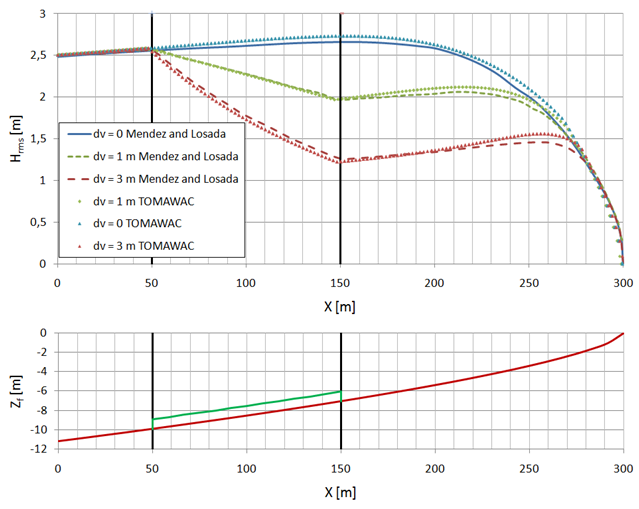
\includegraphics[scale = 0.65]{resdean.png}
 \caption{Comparison of Hrms evolution for numerical wave model (TOMAWAC) and random wave transformation model (Mendez and Losada, 2004) over Dean’s shape profile.}
\label{figresvito}
\end{figure}

% Here is an example of how to include the graph generated by validateTELEMAC.py
% They should be in test_case/img
%\begin{figure} [!h]
%\centering
%\includegraphics[scale=0.3]{../img/mygraph.png}
% \caption{mycaption}\label{mylabel}
%\end{figure}


